% ============================================================================
%  The Legend Challenge: Embedding Ethical Compliance into LLMs through Champion
%  Narratives in the Gender Equality Domain
%  ---------------------------------------------------------------------------
%  Generated by following paper_plan.md (Section Blueprint §4) and pipeline.md.
%  Sections 1 (Introduction) and 2 (Related Work) are intentionally left as
%  \input{} placeholders; the corresponding .tex files exist as separate drafts
%  (paper_draft_abstract_intro.md, paper_draft_related_work.md). Methodology
%  onward is drafted in full below.
% ============================================================================
%Version 3.1 December 2024 See section 11 of the User Manual for version history
%
%%%%%%%%%%%%%%%%%%%%%%%%%%%%%%%%%%%%%%%%%%%%%%%%%%%%%%%%%%%%%%%%%%%%%%
%%                                                                 %%
%% Please do not use \input{...} to include other tex files.       %% % Submit
%your LaTeX manuscript as one .tex document.              %%
%%                                                                 %%
%% All additional figures and files should be attached             %% %
%separately and not embedded in the \TeX\ document itself.       %%
%%                                                                 %%
%%%%%%%%%%%%%%%%%%%%%%%%%%%%%%%%%%%%%%%%%%%%%%%%%%%%%%%%%%%%%%%%%%%%%

%%\documentclass[referee,sn-basic]{sn-jnl}% referee option is meant for double
%line spacing

%%=======================================================%%
%% to print line numbers in the margin use lineno option %%
%%=======================================================%%

%%\documentclass[lineno,pdflatex,sn-basic]{sn-jnl}% Basic Springer Nature
%Reference Style/Chemistry Reference Style

%%=========================================================================================%%
%% the documentclass is set to pdflatex as default. You can delete it if not
%appropriate.  %%
%%=========================================================================================%%

%%\documentclass[sn-basic]{sn-jnl}% Basic Springer Nature Reference
%Style/Chemistry Reference Style

%%Note: the following reference styles support Namedate and Numbered
%referencing. By default the style follows the most common style. To switch
%between the options you can add or remove �Numbered� in the optional
%parenthesis. %The option is available for: sn-basic.bst, sn-chicago.bst%  
 
%%\documentclass[pdflatex,sn-nature]{sn-jnl}% Style for submissions to Nature
%Portfolio journals %\documentclass[pdflatex,sn-basic]{sn-jnl}% Basic Springer
%Nature Reference Style/Chemistry Reference Style
\documentclass[pdflatex, sn-apa]{sn-jnl}% Math and Physical Sciences
%% Numbered Reference Style %\documentclass[pdflatex,sn-mathphys-ay]{sn-jnl}%
%Math and Physical Sciences Author Year Reference Style
%%\documentclass[pdflatex,sn-aps]{sn-jnl}% American Physical Society (APS)
%Reference Style %\documentclass[pdflatex,sn-vancouver-num]{sn-jnl}% Vancouver
%Numbered Reference Style %\documentclass[pdflatex,sn-vancouver-ay]{sn-jnl}%
%Vancouver Author Year Reference Style %\documentclass[pdflatex,sn-apa]{sn-jnl}%
%APA Reference Style %\documentclass[pdflatex,sn-chicago]{sn-jnl}% Chicago-based
%Humanities Reference Style

%%%% Standard Packages %<additional latex packages if required can be included
%here>

\usepackage{graphicx}%
\usepackage{multirow}%
\usepackage{amsmath,amssymb,amsfonts}%
\usepackage{amsthm}%
\usepackage{mathrsfs}%
\usepackage[title]{appendix}%
\usepackage{xcolor}%
\usepackage{textcomp}%
\usepackage{manyfoot}%
\usepackage{booktabs}%
\usepackage{algorithm}%
\usepackage{algorithmicx}%
\usepackage{algpseudocode}%
\usepackage{listings}%
%%%%

%%%%%=============================================================================%%%%
%%%%  Remarks: This template is provided to aid authors with the preparation %%%
%of original research articles intended for submission to journals published %%%
%by Springer Nature. The guidance has been prepared in partnership with %%%
%production teams to conform to Springer Nature technical requirements. %%%
%Editorial and presentation requirements differ among journal portfolios and %%%
%research disciplines. You may find sections in this template are irrelevant %%%
%to your work and are empowered to omit any such section if allowed by the %%%
%journal you intend to submit to. The submission guidelines and policies %%%  of
%the journal take precedence. A detailed User Manual is available in the %%%
%template package for technical guidance.
%%%%%=============================================================================%%%%

%% as per the requirement new theorem styles can be included as shown below
\theoremstyle{thmstyleone}%
\newtheorem{theorem}{Theorem}%  meant for continuous numbers
%%\newtheorem{theorem}{Theorem}[section]% meant for sectionwise numbers %
%optional argument [theorem] produces theorem numbering sequence instead of
%independent numbers for Proposition
\newtheorem{proposition}[theorem]{Proposition}% 
%%\newtheorem{proposition}{Proposition}% to get separate numbers for theorem and
%proposition etc.

\theoremstyle{thmstyletwo}%
\newtheorem{example}{Example}%
\newtheorem{remark}{Remark}%

\theoremstyle{thmstylethree}%
\newtheorem{definition}{Definition}%

\raggedbottom
%%\unnumbered% uncomment this for unnumbered level heads


% ---------- Packages --------------------------------------------------------
\usepackage[T1]{fontenc}
\usepackage[utf8]{inputenc}
\usepackage[british]{babel}
\usepackage{microtype}
\usepackage{geometry}
\geometry{margin=1in}

\usepackage{booktabs}      % Professional table rules
\usepackage{tabularx}      % Flexible tables
\usepackage{array}
\usepackage{multirow}
\usepackage{colortbl}
\usepackage{makecell}

\usepackage{graphicx}
\usepackage{caption}
\usepackage{subcaption}
\usepackage{float}
\usepackage{placeins}

\usepackage{amsmath, amssymb, amsfonts}
\usepackage{mathtools}

\usepackage{pgfplots}
\pgfplotsset{compat=1.18}

\usepackage{xcolor}
\usepackage{hyperref}
\hypersetup{ colorlinks=true, linkcolor=black!50!blue, citecolor=black!50!blue,
  urlcolor=black!50!blue, }
\usepackage[noabbrev]{cleveref}

% Tell cleveref what to call lstlisting environments
\crefname{lstlisting}{listing}{listings}
\Crefname{lstlisting}{Listing}{Listings}

\usepackage{listings}
\usepackage{tcolorbox}
\tcbuselibrary{listings, breakable, skins}

\usepackage{enumitem}
\setlist{nosep, leftmargin=1.25em}
% ---------- Result-highlight macros (from paper-writing/assets/table-style.tex)
\definecolor{bestred}{HTML}{B22222}
\definecolor{secondblue}{HTML}{1F3A8A}
\definecolor{gaingreen}{HTML}{006400}
\definecolor{boxbg}{HTML}{F5F5F5}
\newcommand{\best}[1]{\textcolor{bestred}{\textbf{#1}}}
\newcommand{\second}[1]{\textcolor{secondblue}{\underline{#1}}}
\newcommand{\gain}[1]{\textcolor{gaingreen}{#1}}

% ---------- Listings style for JSON / prompt snippets ----------------------
\lstdefinelanguage{json}{ basicstyle=\ttfamily\footnotesize,
  showstringspaces=false, breaklines=true, frame=none, literate=
  *{0}{{{\color{black!60}0}}}{1} {1}{{{\color{black!60}1}}}{1}
  {2}{{{\color{black!60}2}}}{1} {3}{{{\color{black!60}3}}}{1}
  {4}{{{\color{black!60}4}}}{1} {5}{{{\color{black!60}5}}}{1}
  {6}{{{\color{black!60}6}}}{1} {7}{{{\color{black!60}7}}}{1}
  {8}{{{\color{black!60}8}}}{1} {9}{{{\color{black!60}9}}}{1}, } \lstset{
  basicstyle=\ttfamily\footnotesize, breaklines=true, columns=fullflexible,
  showstringspaces=false, }

\newtcolorbox{promptbox}[1][]{ colback=boxbg, colframe=black!40,
  fonttitle=\bfseries, breakable, sharp corners, boxrule=0.4pt, left=4pt,
  right=4pt, top=4pt, bottom=4pt, #1 }

% ---------- Custom macros --------------------------------------------------
\newcommand{\modelbase}{\texttt{base}}
\newcommand{\modellegends}{\texttt{tuned-legends}}
\newcommand{\modelreg}{\texttt{tuned-regulation}}
\newcommand{\bm}{\textbf}



\begin{document}

\title[The Legend Challenge: Embedding Ethical Compliance into LLMs through Champion Narratives in the Gender Equality Domain]{The Legend Challenge: Embedding Ethical Compliance into LLMs through Champion Narratives in the Gender Equality Domain}

%%=============================================================%%
%% GivenName    -> \fnm{Joergen W.} % Particle -> \spfx{van der} -> surname
%prefix % FamilyName   -> \sur{Ploeg} % Suffix   -> \sfx{IV} %
%\author*[1,2]{\fnm{Joergen W.} \spfx{van der} \sur{Ploeg} %
%\sfx{IV}}\email{iauthor@gmail.com}
%%=============================================================%%

\author*[1]{\fnm{Fatmir} \sur{Bylyshi}}\email{fatmir.bylyshi@studenti.unimi.it}
\equalcont{These authors contributed equally to this work.}

\author*[1]{\fnm{Ouardi} \sur{Ilyass}}\email{ilyass.ouardi@studenti.unimi.it}
\equalcont{These authors contributed equally to this work.}

% \author[1,2]{\fnm{Third} \sur{Author}}\email{iiiauthor@gmail.com}
% \equalcont{These authors contributed equally to this work.}

\affil*[1]{\orgdiv{Department of Computer Science}, \orgname{University of
Milan}, \orgaddress{\street{Via Celoria, 20}, \city{Milan}, \postcode{20134},
\country{Italy}}}

%%==================================%%
%% Sample for unstructured abstract %%
%%==================================%%

% \abstract{Large companies operating under increasingly complex sustainability and gender-equality regulations face a structural conflict between cost-optimisation incentives, which AI systems are designed to maximise, and the social-cost considerations that regulation requires them to honour. Sargsyan and Damiani (2025) characterise this tension as a compliance paradox and propose that ethical behaviour can be embedded into Large Language Models (LLMs) ex ante, by exposing the model to synthetic "champion" profiles — narratively rich legends that incarnate regulatory compliance — rather than ex post, through audit. This paper operationalises that proposal in the gender-equality domain. We select the EU Gender Equality Strategy 2020-2025 as the regulatory anchor and design a four-axis prompt-engineering protocol — absolute thematic verticality, internal reflection on compliance gaps, high technical specificity with explicit regulatory citations, and middle-management protagonists — to generate legends that mirror the implementation context flagged as the locus of conflict in Sargsyan and Damiani (2025). The legends and the regulation text are converted into a parallel pair of size-matched JSONL Question-Answering datasets through an adapted SustainableQA pipeline (Lan et al., 2025), and two specialised model variants are trained on the FineTuneDB platform on top of the GPT-4o-2024-08-06 backbone. We then evaluate the base model and the two tuned variants on GenderEqGLUE, a five-task benchmark we construct in the LexGLUE tradition (Chalkidis et al., 2022) for the gender-equality domain. The aggregate ranking is tuned-regulation ≈ tuned-legends > base (GenderEqGLUE Scores 0.937, 0.931, and 0.902 respectively), with the two fine-tuned models splitting the per-task wins 3–3. Per-task and per-slice analysis reveals a qualitative complementarity between the two fine-tuning regimes: the legend-tuned model wins the central compliance-recognition task (GE-NLI), the compliant-action prediction task (GE-NEXT) — the first task on which the legend hypothesis achieves formal McNemar significance — and achieves perfect gender-parity on WinoBias (GE-WSC), while the regulation-tuned model dominates ontology classification (GE-CLS) and short-span factoid extraction (GE-QA). We interpret this as evidence that legends teach compliance recognition and compliant-action selection while regulatory text teaches violation detection and ontology recognition, and that the two fine-tuning regimes are complementary inductive biases rather than strict alternatives.}


\abstract{\citet{sargsyan2025legends} proposed that fine-tuning large language
models on \emph{legends}, synthetic narrative exemplars of compliant behaviour,
might embed regulatory ethics more effectively than fine-tuning on the
underlying regulatory text, but they offered neither an empirical test nor a
measurement instrument. This paper supplies preliminary versions of both. We
compare legend-based fine-tuning against regulation-text fine-tuning on a
single regulation (the EU Gender Equality Strategy 2020--2025) and a single
backbone (\texttt{gpt-4o-2024-08-06}), holding the system prompt, training
format, and JSONL line count approximately constant. To make the comparison
measurable we introduce \textbf{GenderEqGLUE}, a five-task benchmark
(GE-CLS, GE-NLI, GE-QA, GE-WSC, GE-NEXT) adapted from GLUE and SuperGLUE
templates and built on a held-out Common Evaluation Base of 217 EU passages.
Because FineTuneDB Studio exposes neither logits nor model internals, we also
introduce \textbf{Counterfactual Input Probing (CIP)}, a small-scale
behavioural protocol. On the aggregate GenderEqGLUE Score, \modelreg{} leads at
0.938, \modellegends{} follows at 0.926, and \modelbase{} trails at 0.904; the
two fine-tuned models split per-task wins 3--3. \modellegends{} is the
strongest of the three on GE-NEXT, the only task where a pairwise McNemar
contrast reaches $p<0.05$ ($p=0.031$ against the base, $n=150$). The data are
\emph{compatible with} the reading that the two regimes teach complementary
competences, but the test-set sizes are small enough, and the cross-task
patterns inconsistent enough, that the present results are best understood as
preliminary observations rather than as a settled hierarchy. We treat the
contribution of this work as the construction of the benchmark and probing
instruments themselves, on which a properly powered follow-up could deliver
the stronger evidence the original hypothesis demands.}

\keywords{ethical AI, regulatory compliance, gender equality, large language models, fine-tuning, legends, GLUE, GenderEqGLUE, explainability, EU Gender Equality Strategy}

\maketitle

% ============================================================================
% §1 - INTRODUCTION
% ============================================================================
\section{Introduction}
\label{sec:intro}

\begin{figure}[t]
\centering
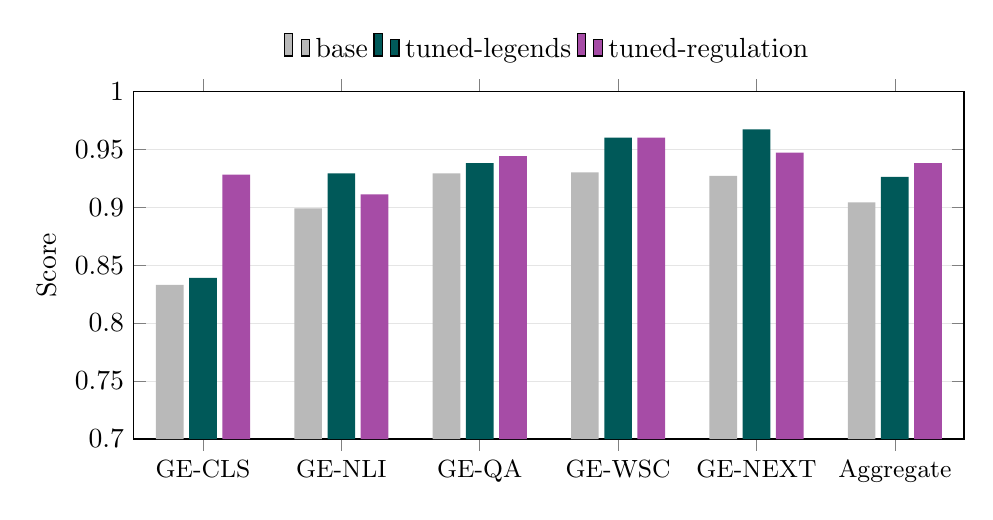
\begin{tikzpicture}
\begin{axis}[ ybar, width=\linewidth, height=6cm, bar width=10pt, ymin=0.70,
    ymax=1.0, ylabel={Score}, ytick={0.70,0.75,0.80,0.85,0.90,0.95,1.0},
    symbolic x coords={GE-CLS,GE-NLI,GE-QA,GE-WSC,GE-NEXT,Aggregate},
    xtick=data, x tick label style={font=\small}, legend style={at={(0.5,1.05)},
    anchor=south, legend columns=3, draw=none}, enlarge x limits=0.10,
    ymajorgrids, major grid style={gray!20}, ]
\addplot[fill=gray!55,draw=none] coordinates
    {(GE-CLS,0.833)(GE-NLI,0.899)(GE-QA,0.929)(GE-WSC,0.930)(GE-NEXT,0.927)(Aggregate,0.904)};
\addplot[fill=teal!70!black,draw=none] coordinates
    {(GE-CLS,0.839)(GE-NLI,0.929)(GE-QA,0.938)(GE-WSC,0.960)(GE-NEXT,0.967)(Aggregate,0.926)};
\addplot[fill=violet!70,draw=none] coordinates
    {(GE-CLS,0.928)(GE-NLI,0.911)(GE-QA,0.944)(GE-WSC,0.960)(GE-NEXT,0.947)(Aggregate,0.938)};
\legend{base, tuned-legends, tuned-regulation}
\end{axis}
\end{tikzpicture}
\caption{Per-task scores for the three models. The two fine-tuned regimes
split the five tasks; the aggregate gap between them is 1.2 points, smaller
than the bootstrap confidence intervals on most individual tasks.}
\label{fig:teaser}
\end{figure}

Large language models are increasingly delegated middle-management decisions
in domains directly governed by regulation. \citet{sargsyan2025legends}
characterise a structural conflict in such deployments: cost-optimisation
incentives, on which AI systems are typically tuned, compete with the
social-cost considerations that regulation imposes, and the result is a
governance vulnerability that post-hoc filtering does not adequately close.
They propose embedding compliance \emph{ex ante} into the model's training
signal, specifically through \emph{legends}: synthetic narrative exemplars
(``champion profiles'') of individuals or institutions whose behaviour
incarnates regulatory compliance. The intuition is that a model fine-tuned on
legends learns compliance as a capacity exercised over novel inputs, rather
than as a lookup against memorised regulatory vocabulary. The proposal is
specific and normatively appealing, but the original work supplies neither an
empirical test of the proposition that legend fine-tuning differs measurably
from regulation-text fine-tuning, nor a measurement instrument on which the
claim could be evaluated.

Two converging gaps prevent existing literature from supplying either.
First, the standard NLU benchmark suites, GLUE \citep{wang2018glue} and
SuperGLUE \citep{wang2019superglue}, are deliberately domain-agnostic: they
do not probe whether a model recognises compliance, selects compliant
actions, or generalises across the thematic pillars of a particular
regulation. Adapting their templates to a single named regulation has not, to
our knowledge, been attempted in the gender-equality domain. Second, the
standard explainability tooling that would let a researcher inspect
\emph{how} a fine-tuned model arrived at a decision, SHAP
\citep{lundberg2017shap}, LIME \citep{ribeiro2016lime}, Integrated Gradients
\citep{sundararajan2017ig}, attention rollout \citep{abnar2020rollout},
requires gradients, logits, or hundreds of model calls per instance. The
industrial fine-tuning platform on which this study runs, FineTuneDB Studio,
exposes none of these; generated text is the sole observable.

This paper develops three artefacts that, taken together, support a
preliminary test of the hypothesis under matched fine-tuning conditions.
\emph{First}, a SustainableQA-derived
\citep{wattenberg2025sustainableqa} pipeline converts regulatory text and
synthetic legends into matched JSONL fine-tuning corpora that share system
prompt, chat format, and approximate line count. \emph{Second},
\textbf{GenderEqGLUE} adapts five canonical GLUE/SuperGLUE templates,
classification, NLI, reading comprehension, coreference, and commonsense
action selection, to the EU Gender Equality Strategy 2020--2025, anchored in
a held-out Common Evaluation Base. \emph{Third},
\textbf{Counterfactual Input Probing (CIP)} is a behavioural-only protocol
that subjects one prediction per pillar to three controlled input variants
(original, keyword-stripped, adversarially framed); we use it as the
methodology the closed-platform access constraint admits, not as a substitute
for the gradient-based tools it forecloses.

We adopt the following as the minimal defensible reading of our results.
The two fine-tuning regimes produce models with patterns of strengths and
weaknesses that differ across the five tasks: \modelreg{} leads the
aggregate (0.938) and dominates the tasks that map most directly to the
regulation's lexical and ontological structure (GE-CLS, GE-QA short-span);
\modellegends{} leads on GE-NEXT and GE-NLI, the two tasks designated
\emph{a priori} as the central tests of the Sargsyan-Damiani hypothesis,
with GE-NEXT the only pairwise contrast in the study to clear $p<0.05$. We
read this as suggestive of complementarity between the two regimes; we do
not read it as a settled architectural finding, both because most pairwise
gaps remain below significance at the present test-set sizes and because the
CIP probing sample ($n=15$) is too small to support the kind of qualitative
follow-up the hypothesis ultimately requires.

The remainder of the paper is structured as follows. \Cref{sec:related}
situates the work against prior approaches to embedding ethics in LLMs,
domain-agnostic NLU benchmarks, domain QA-generation pipelines, and
explainability under closed access. \Cref{sec:method} describes the
dataset-construction pipeline. \Cref{sec:benchmark} details the construction
of the GenderEqGLUE benchmark. \Cref{sec:results} reports headline results
and per-task breakdowns. \Cref{sec:cip} presents the CIP protocol and its
qualitative observations. \Cref{sec:discussion} discusses the
complementarity reading and its limits; \Cref{sec:limitations} records the
limitations of the test-set sizes, single-backbone scope, and closed-platform
access regime; and \Cref{sec:conclusion} concludes.

% ============================================================================
% §2 - RELATED WORK
% ============================================================================
\section{Related Work}
\label{sec:related}

\paragraph{Embedding ethics in LLMs.}
Regulation can be integrated into model behaviour through several routes.
One translates regulations into machine-readable representations: the X2RL
semantic regulatory format \citep{mclaughlin2021x2rl} and Denmark's
digital-ready legislation initiative \citep{motzfeldt2018digital} exemplify
this direction, while pilots on U.S.\ public-benefits policy under the
Rules-as-Code paradigm suggest that LLMs can support such pipelines but
require extensive prompting and human oversight to preserve equity
\citep{naumova2023responsibility}. A second route fine-tunes models on
regulatory text directly: IBM's Alignment Studio
\citep{achintalwar2024alignment} aligns LLMs to contextual regulations using
business-conduct guidelines, and its authors report limitations they
attribute to the literal-textual character of the training signal,
limitations the present paper is in part a controlled study of.

\paragraph{NLU benchmarks and their domain-agnostic limit.}
GLUE \citep{wang2018glue} and SuperGLUE \citep{wang2019superglue} provide
composite scores across single-sentence classification, NLI, reading
comprehension, and commonsense reasoning, with constituent datasets
including SST-2, MNLI, RTE, SQuAD \citep{rajpurkar2016squad}, BoolQ
\citep{clark2019boolq}, WSC, COPA \citep{roemmele2011copa}, and the
gender-aware WinoBias coreference probe \citep{zhao2018winobias}. Their
design choice is deliberately domain-agnostic; a high GLUE score reflects
generic linguistic competence, not reasoning over a specific regulation's
structure. Recent benchmarks address legal and corporate domains, but none,
to our knowledge, targets the competences the Sargsyan-Damiani hypothesis
foregrounds. GenderEqGLUE adapts the five canonical templates one-to-one to
the EU Gender Equality Strategy, anchors them in held-out passages, and adds
a four-type distractor typology to its action-selection task.

\paragraph{Domain QA-generation pipelines.}
\textbf{SustainableQA} \citep{wattenberg2025sustainableqa} is a scalable
pipeline for generating Q\&A pairs from corporate sustainability reports,
combining semantic-chunk classification, hybrid span extraction, and
per-span factoid plus non-factoid question generation. Our pipeline
preserves its overall architecture but replaces the multi-stage
NER\,+\,regex span extractor with a single LLM-driven extractor (justified
by the cleaner structure of regulatory and legend text relative to
corporate filings) and omits table handling.

\paragraph{Explainability under closed access.}
Standard explainability tools for large neural models, SHAP, LIME,
Integrated Gradients, and attention rollout, all assume model access that
FineTuneDB Studio does not provide. The CIP protocol introduced here
borrows LIME's perturbation logic and applies it strictly at the text level
on a small, hand-designed variant set; it is positioned as the methodology
this access constraint admits, not as a substitute for the gradient-based
tools it forecloses.

% ============================================================================
% §3 - METHODOLOGY
% ============================================================================
\section{Methodology: Dataset-Construction Pipeline}
\label{sec:method}

The empirical test requires two fine-tuning corpora that differ only in
whether their content is regulatory text or narrative exemplars derived
from that text. The pipeline described here is the procedural instrument
that produces these matched corpora.

\begin{figure}[!ht]
  \centering
  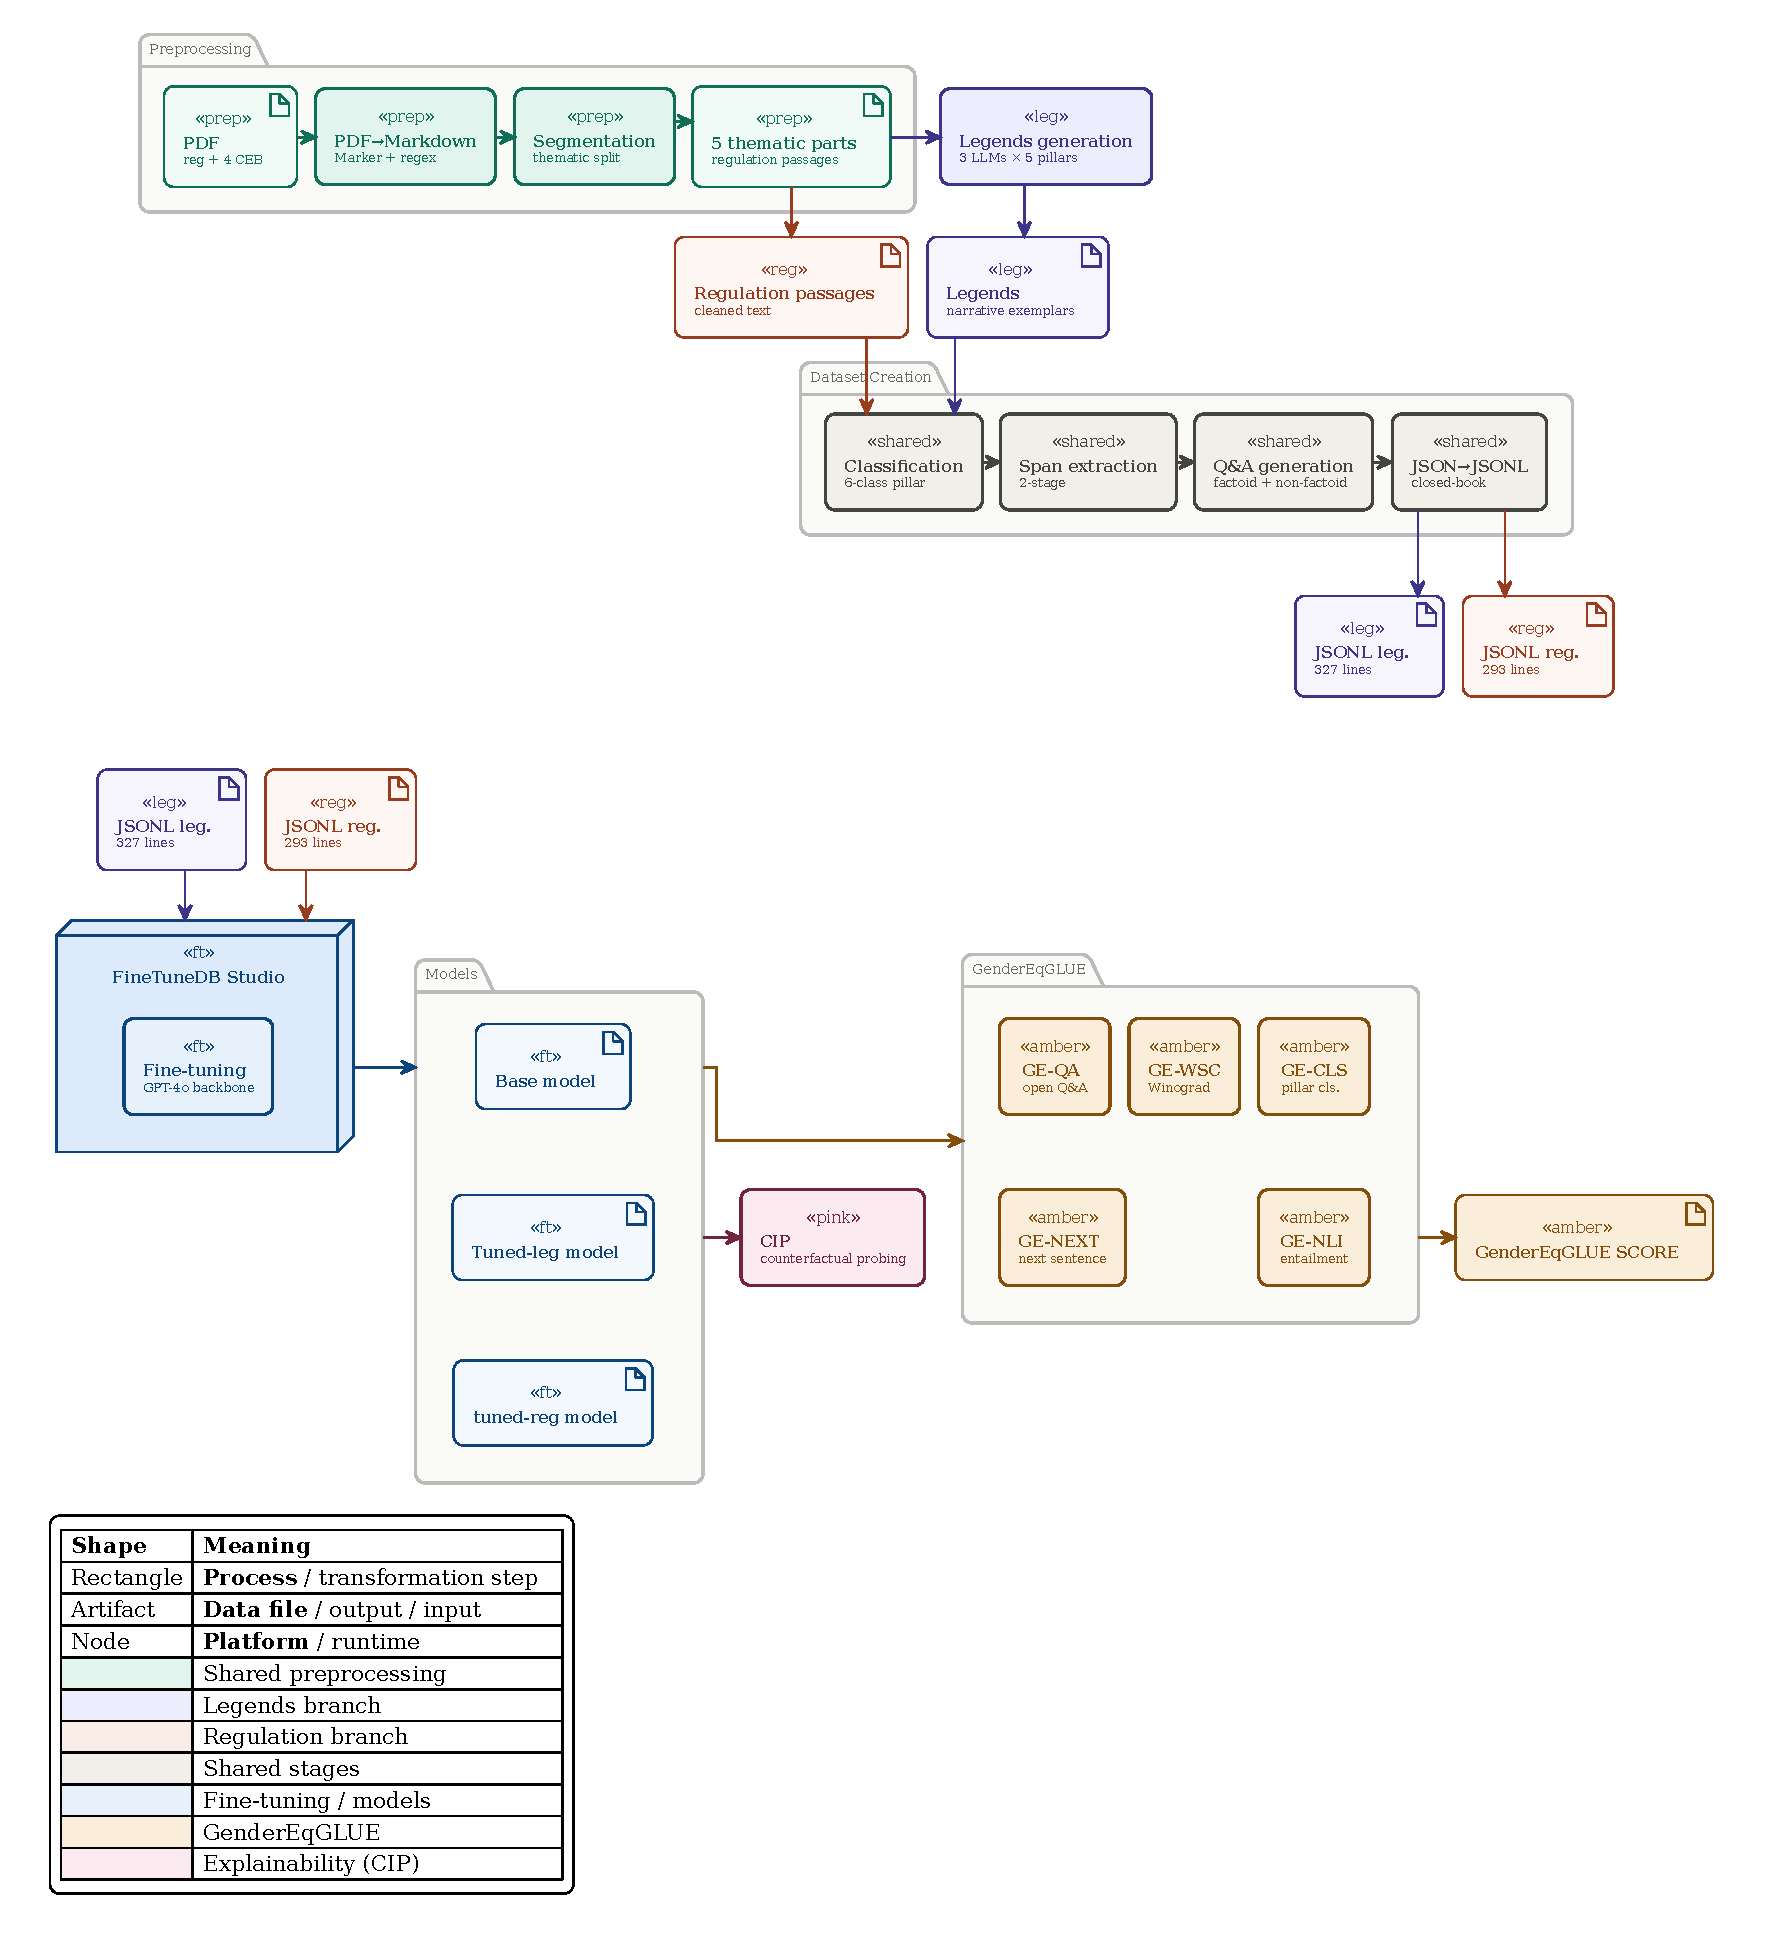
\includegraphics[width=\textwidth]{pipeline_combined.pdf}
  \caption{End-to-end pipeline. The legends branch and the regulation
    branch traverse identical preprocessing, classification, span
    extraction, and Q\&A-generation stages, differing only in source
    content. The resulting JSONL files share system prompt, chat format,
    and approximate line count, isolating corpus content as the
    experimental variable.}
  \label{fig:pipeline}
\end{figure}

\Cref{fig:pipeline} summarises the pipeline. It adapts the SustainableQA
framework \citep{wattenberg2025sustainableqa} to the regulatory-compliance
setting through seven stages: preprocessing (PDF$\to$Markdown plus regex
cleaning), legends generation, six-class pillar classification, two-stage
span extraction, factoid plus non-factoid Q\&A generation, and fine-tuning
of the GPT-4o backbone on FineTuneDB Studio. Both branches share a single
system prompt and emerge as parallel JSONL files of approximately matched
size (327 vs 293 lines).

\paragraph{Preprocessing.}
The Strategy is published as a layout-dense PDF containing footnotes,
URLs, image references, and rendering artefacts. The Marker library
\citep{paruchuri2024marker} converts the PDF to Markdown while preserving
heading hierarchy; a regex pass removes footnote markers, image
references, URLs, LaTeX artefacts, and consecutive blank lines. Cleaning
reduces the document from 64{,}703 to 45{,}697 characters (29.4\%) while
preserving all 16 section headings and every numerical commitment. The
cleaned document is segmented in two stages: top-level Markdown headings
partition it into five thematic parts (one per substantive pillar of the
Strategy, plus an ``unknown'' rejection class); sub-headings and a
350-word maximum further split each part at paragraph boundaries.

\paragraph{Legends generation.}
The Sargsyan-Damiani hypothesis requires narrative exemplars instantiating
a four-beat arc (\emph{identify gap}~$\to$~\emph{design measure}~$\to$
\emph{implement}~$\to$~\emph{measurable outcome}). Three frontier LLMs
(Gemini, Microsoft Copilot, OpenAI ChatGPT) each generate five legends,
one per pillar, conditioned on the corresponding thematic part and on an
identical system prompt fixing the legend format (title, setting, 3--5
named characters, 400--600 word narrative with at least one direct-speech
dialogue, measurable outcome, explicit acknowledgement of the Strategy).
Multi-LLM mixing reduces overfitting to any single generator's idioms.
The full system prompt is documented in the reproducibility appendix
(\Cref{app:reproducibility}). The legend pool is small (15 narratives) but
yields 327 closed-book Q\&A pairs after the downstream stages, of
comparable line count to the 293 pairs derived from the regulation text.

\paragraph{Pillar classification.}
Each passage from the segmentation stage is classified by Gemini~3 Pro
into one of six categories: the five substantive pillars
(\texttt{violence\_stereotypes}, \texttt{equal\_economy},
\texttt{leadership\_participation},
\texttt{mainstreaming\_intersectionality}, \texttt{funding\_global\_action})
plus \texttt{unknown}, which captures administrative metadata, headers,
and off-topic passages. A single classifier and a single taxonomy are
reused across the regulation-text JSONL, the legend JSONL, and the
held-out benchmark pool described in \Cref{sec:bench:ceb}, so that pillar
labels carry the same meaning in training and at evaluation. The
classification prompt is reproduced in the reproducibility appendix.

\paragraph{Two-stage span extraction.}
Factoid Q\&A generation requires short verbatim spans usable as gold
answers. Stage~1 is a high-recall LLM-driven extractor: Gemini~3 Pro
identifies every verbatim span aligning with a pillar, legal directive,
or socio-economic target (typical length 1--5 words; up to 8 for complex
named entities). Stage~2 verifies that each candidate appears verbatim in
the source, filters redundancies, and clusters the survivors into
thematic groups with an \texttt{Individual} fallback for unique spans.
The two-stage decomposition isolates recall and uniqueness; the clustered
output also feeds the non-factoid generator.

\paragraph{Q\&A generation.}
Two parallel LLM calls (Gemini 3 Pro) are made per passage. The factoid
generator takes verified spans and produces questions whose answer is
exactly one verbatim span, validated against a three-rule self-correction
checklist (verbatim answer, context-only support, natural phrasing). The
non-factoid generator produces descriptive (1--4 sentence) answers grounded
in the passage, validated by a four-rule checklist (genuinely non-factoid,
distinct from siblings, fully answerable from context, accurate summary).
Both generators emit JSON; failed pairs are discarded rather than retried,
moving quality control inside the generation prompt.

\paragraph{Fine-tuning.}
Each JSONL line carries three chat turns: an identical system prompt
anchoring the model in the gender-equality domain, a user question, and a
gold answer. Both runs use \texttt{gpt-4o-2024-08-06}, fine-tuned via the
FineTuneDB Studio interface, which controls hyperparameters, optimiser,
learning-rate schedule, and termination criteria identically across the
two runs. The legends JSONL contains 327 lines (199 non-factoid + 128
factoid; 45 \texttt{unknown} chunks skipped); the regulation JSONL
contains 293 lines (184 non-factoid + 109 factoid; 5 \texttt{unknown}
skipped). Pillar distributions across the two corpora are necessarily
unequal because they reflect the underlying source content, and we treat
this as a property of the comparison rather than an enforced invariant.
The closed-platform access regime, while it controls hyperparameters, is
also the constraint that motivates \Cref{sec:cip}.

% ============================================================================
% §4 - BENCHMARK
% ============================================================================
\section{GenderEqGLUE: A Regulatory-Compliance Reasoning Benchmark}
\label{sec:benchmark}

The standard NLU benchmark suites are domain-agnostic and do not probe
regulatory-compliance reasoning. GenderEqGLUE adapts the five canonical
GLUE/SuperGLUE task templates one-to-one to the EU Gender Equality
Strategy 2020--2025. \Cref{tab:tasks} summarises the five tasks.

\begin{table}[h]
\centering
\caption{GenderEqGLUE task overview. The first three tasks share a Common
Evaluation Base (CEB) of 217 EU passages held out from fine-tuning;
GE-WSC uses WinoBias \citep{zhao2018winobias} as-is; GE-NEXT is
constructed from scratch.}
\label{tab:tasks}
\small
\begin{tabularx}{\linewidth}{@{}lXllX@{}}
\toprule
Task    & Description                          & GLUE analogue   & Source                              & Metric                       \\
\midrule
GE-CLS  & Pillar classification (6-class)      & SST-2           & CEB-CLS (72 passages)               & Macro-F1                     \\
GE-NLI  & Compliance entailment (3-class)      & MNLI / RTE      & CEB-NLI                             & Accuracy                     \\
GE-QA   & Regulation reading comprehension     & SQuAD / BoolQ   & CEB-QA (open-book)                  & F1 / EM, accuracy            \\
GE-WSC  & Stereotype-aware coreference         & WSC / Winogender& WinoBias                            & Accuracy + parity            \\
GE-NEXT & Compliant-action selection (4-choice)& COPA            & Curated vignettes                   & Accuracy                     \\
\bottomrule
\end{tabularx}
\end{table}

The aggregate \textbf{GenderEqGLUE Score} is the unweighted arithmetic
mean of the five per-task headline metrics.

\subsection{Common Evaluation Base}
\label{sec:bench:ceb}

Three of the five tasks (GE-CLS, GE-NLI, GE-QA) draw their items from a
single \textbf{Common Evaluation Base} of 217 EU passages held out from
both fine-tuning corpora. The CEB is constructed from four EU documents
thematically contiguous with the Strategy but absent from the training
corpora: the Roadmap for Women's Rights (2025), Gender Action Plan III
(2021--2025), Council Conclusions on Closing the Gender Pay Gap (June
2019), and Directive (EU)~2022/2381 on the gender balance among
directors of listed companies. These documents pass through the same
preprocessing pipeline as the Strategy, are classified by the same
six-class pillar classifier, and are stratified into three disjoint
subsets (CEB-CLS, CEB-QA, CEB-NLI) by two sequential calls to
\texttt{train\_test\_split} with \texttt{random\_state=42}.
\Cref{tab:ceb} reports the per-pillar distribution.

\begin{table}[h]
\centering
\caption{Common Evaluation Base: per-pillar distribution after stratified
1/3 split. The \texttt{unknown} class is excluded from substantive task
construction but retained as a GE-CLS rejection target.}
\label{tab:ceb}
\small
\begin{tabular}{@{}lrrrr@{}}
\toprule
Pillar                                & Pool & CLS & QA & NLI \\
\midrule
\texttt{violence\_stereotypes}        & 72   & 24  & 24 & 24  \\
\texttt{leadership\_participation}    & 45   & 15  & 15 & 15  \\
\texttt{funding\_global\_action}      & 21   &  7  &  7 &  7  \\
\texttt{equal\_economy}               & 18   &  6  &  6 &  6  \\
\texttt{mainstreaming\_intersectionality} & 11 & 4  &  3 &  4  \\
\texttt{unknown}                      & 50   & 16  & 17 & 17  \\
\midrule
\textbf{Total}                        & 217  & 72  & 72 & 73  \\
\bottomrule
\end{tabular}
\end{table}

\subsection{The Five Tasks}
\label{sec:bench:tasks}

\paragraph{GE-CLS (pillar classification).}
A six-way classification of a passage into one of the five pillars or
\texttt{unknown}. The headline metric is Macro-F1; per-class F1 on the
three minority pillars ($n<30$) is flagged as low-confidence. CEB-CLS
(72 passages) is used directly. GE-CLS generalises SST-2's single-input
categorical mapping from binary sentiment to six-way thematic
classification, evaluating internalisation of the regulation's pillar
ontology.

\paragraph{GE-NLI (compliance entailment).}
Given a scenario (premise) and a regulatory clause (hypothesis), the
model decides whether the scenario entails, contradicts, or is neutral
with respect to the clause. Headline metric: accuracy. GE-NLI is the
\emph{a priori} central task for the Sargsyan-Damiani hypothesis: it
measures compliance recognition directly. The dataset contains 168
triples (56 per class), generated from the 56 substantive CEB-NLI
passages. For each passage, one regulatory clause is extracted as the
hypothesis (length 8--35 words); a compliant scenario is generated as
the entailment premise, with sector and country rotating cyclically; the
compliant premise is then perturbed along a single quantitative or
factual axis (numeric inversion, policy reversal, threshold undershoot,
mechanism removal, scope reduction, deadline miss) to yield the
contradiction triple; and the compliant premise is paired with a
hypothesis from a different pillar to yield the neutral triple. Class
balance and deduplication are verified at the end.

\paragraph{GE-QA (regulation reading comprehension).}
Given an EU regulatory passage and a question, produce an answer. The
task has two sub-tasks: GE-QA-Factoid (SQuAD-style short-span; F1 and EM
reported, with EM as a stricter diagnostic) and GE-QA-Bool (yes/no
accuracy). GE-QA is the benchmark's only \emph{open-book} task. Factoid
items reuse the span extractor and factoid generator of
\Cref{sec:method} on CEB-QA, restricted to self-contained questions and
spans of at most 7 words. Bool items are constructed by direct
paraphrase (passage claim rewritten as a polar question; gold=yes) and
perturbed claim (a single quantitative or scope dimension inverted;
gold=no), balanced 50/50.

\paragraph{GE-WSC (stereotype-aware coreference).}
WinoBias \citep{zhao2018winobias} is used \emph{as-is} from the
HuggingFace Hub with all four subsets preserved unmodified. The task
reports accuracy averaged across the four subsets and a
\textbf{Gender Parity Score} $|\text{acc}_{\text{pro}} -
\text{acc}_{\text{anti}}|$, where a value of 0 indicates
stereotype-invariant behaviour. The choice to preserve WinoBias keeps
GE-WSC comparable with the broader bias-evaluation literature, at the
cost of domain mismatch with the rest of the benchmark; the bias
originates in pretraining distribution rather than in either fine-tuning
corpus, so substantial accuracy improvement is not expected and the
parity diagnostic is the quantity of interest.

\paragraph{GE-NEXT (compliant-action selection).}
Given a vignette describing a quantified gender-equality gap, the model
selects the next-step action most consistent with the Strategy. Each
item presents a 2--4 sentence vignette identifying a fictional
middle-management protagonist, an organisational context, a quantified
gap, and four candidate actions: one substantive-compliant (gold), one
\textbf{performative} (symbolic gesture without measurable KPIs), one
\textbf{cost-optimising} (defers or minimises remediation at the
expense of the regulatory objective), and one \textbf{orthogonal}
(plausible action addressing a different gender-equality concern). The
benchmark contains 150 items (30 per pillar), constructed from CEB
regulatory clauses with options shuffled under a fixed seed and a 20\%
manual quality review. GE-NEXT is the most direct probe of the
compliance-versus-cost arbitrage; its gold options mirror the
four-beat narrative arc of the legend training signal.

\subsection{Aggregate Score and Statistical Protocol}
\label{sec:bench:protocol}

For each model we report the five per-task headline metrics and their
unweighted arithmetic mean. Bootstrap 95\% confidence intervals (2000
resamples, \texttt{seed=42}) are reported on each headline metric;
pairwise model comparisons use McNemar's exact-binomial test on per-item
correctness (the exact variant chosen because discordant counts $b+c$
remain small). Per-class, per-pillar, and per-construction-method
diagnostics are reported alongside the aggregates so that compressed
gaps can be interpreted at the level of the items they arise from.

\FloatBarrier

% ============================================================================
% §5 - RESULTS
% ============================================================================
\section{Results}
\label{sec:results}

\subsection{Headline Scores}
\label{sec:results:headline}

\Cref{tab:headline} reports the five per-task headline metrics and the
aggregate GenderEqGLUE Score; \Cref{tab:wins} summarises the per-task
wins.

\begin{table}[h]
\centering
\caption{Per-task headline metrics and aggregate GenderEqGLUE Score.
\best{Red bold}: per-column maximum. Ties on GE-WSC are bolded for both
fine-tuned regimes.}
\label{tab:headline}
\small
\begin{tabular}{@{}lcccccc@{}}
\toprule
Model            & GE-CLS         & GE-NLI         & GE-QA          & GE-WSC         & GE-NEXT        & \textbf{GenderEqGLUE} \\
                 & (Macro-F1)     & (Accuracy)     & ((F1+Bool)/2)  & (Accuracy)     & (Accuracy)     & (mean)                \\
\midrule
\modelbase       & 0.833          & 0.899          & 0.929          & 0.930          & 0.927          & 0.904                 \\
\modellegends    & 0.839          & \best{0.929}   & 0.938          & \best{0.960}   & \best{0.967}   & 0.926                 \\
\modelreg        & \best{0.928}   & 0.911          & \best{0.944}   & \best{0.960}   & 0.947          & \best{0.938}          \\
\bottomrule
\end{tabular}
\end{table}

\begin{table}[h]
\centering
\caption{Wins per task. The two fine-tuned models split the benchmark
3--3; the base does not top any column.}
\label{tab:wins}
\small
\begin{tabular}{@{}llc@{}}
\toprule
Model            & Tasks won                                         & Wins / 5 \\
\midrule
\modelreg        & GE-CLS, GE-QA, GE-WSC (tied)                      & 3 / 5    \\
\modellegends    & GE-NLI, GE-NEXT, GE-WSC (tied)                    & 3 / 5    \\
\modelbase       & ---                                               & 0 / 5    \\
\bottomrule
\end{tabular}
\end{table}

\modelreg{} achieves the highest aggregate score (0.938), with a margin
of $+3.4$ points over the base and $+1.2$ points over \modellegends.
Both fine-tuned models improve over the base on every task. The 1.2-point
aggregate gap between the two tuned regimes is smaller than the
bootstrap confidence interval on most individual tasks, and we therefore
read the per-task wins distribution as the more informative summary:
\modelreg{} leads on the tasks that map directly to the regulation's
ontology and short-span factual structure (GE-CLS, GE-QA);
\modellegends{} leads on the two tasks designated \emph{a priori} as
central tests of the hypothesis (GE-NLI, GE-NEXT).

\subsection{GE-NEXT Distractor Analysis}
\label{sec:results:distractor}

\Cref{tab:distractor} reports the per-distractor-type error rate on
GE-NEXT ($n=150$).

\begin{table}[h]
\centering
\caption{GE-NEXT per-distractor-type error rate (share of each model's
wrong picks; absolute counts in parentheses). \modelbase{} makes 11
wrong picks; \modelreg{} makes 8; \modellegends{} makes 5.}
\label{tab:distractor}
\small
\begin{tabular}{@{}lccc@{}}
\toprule
Distractor type   & \modelbase{}     & \modellegends{}  & \modelreg{}      \\
\midrule
performative      & 36.36\% (4/11)   & 40.00\% (2/5)    & 37.50\% (3/8)    \\
cost-optimising   & 18.18\% (2/11)   & 20.00\% (1/5)    & 12.50\% (1/8)    \\
\rowcolor{boxbg}
orthogonal        & \best{45.45\% (5/11)} & 40.00\% (2/5) & \best{50.00\% (4/8)} \\
\bottomrule
\end{tabular}
\end{table}

Three patterns emerge from these absolute counts, all of which should be
read against the small underlying error totals. Orthogonal is the
modal failure mode for all three models (5/11, 2/5, 4/8); when models
are wrong they most often select a substantive-looking action addressed
to a different gender-equality concern than the one in the vignette.
Performative errors are present at broadly similar rates across the
three regimes (4/11, 2/5, 3/8). Cost-optimising is rejected most
reliably by all three models, including the base. The pairwise McNemar
contrast between \modelbase{} and \modellegends{} reaches $p=0.031$ on
GE-NEXT ($b=0$, $c=6$), making it the only pairwise contrast in the
study to clear $p<0.05$. We read this as the strongest single piece of
evidence in the benchmark for a legends-specific effect, while noting
that resolving the legends-versus-regulation gap on the same task would
require approximately 350--500 items at the observed effect size.

\subsection{Cross-Task Pillar Effects}
\label{sec:results:pillars}

\Cref{tab:pillars} reports per-pillar performance gains relative to the
base for the four tasks where pillar labels are defined (GE-WSC is
excluded as it uses WinoBias professions).

\begin{table}[h]
\centering
\caption{Cross-task pillar effects. Each cell is the per-pillar
performance gain (winning fine-tuned model $-$ base) on the indicated
task. Gains on the minority pillars (\texttt{equal\_economy},
\texttt{mainstreaming\_intersectionality}) should be read with their
small support sizes ($n=6$, $n=4$) in mind.}
\label{tab:pillars}
\small
\begin{tabular}{@{}lrrrr@{}}
\toprule
Pillar                                & GE-CLS        & GE-NLI        & GE-QA         & GE-NEXT       \\
                                      & (reg $-$ base)& (legends $-$ base) & (reg $-$ base) & (legends $-$ base) \\
\midrule
\texttt{violence\_stereotypes}        & $+0.045$      & $+0.028$      & $+0.023$      & $+0.067$      \\
\texttt{equal\_economy}               & $+0.167$      & $+0.111$      & $+0.029$      & $+0.067$      \\
\texttt{leadership\_participation}    & $+0.000$      & $+0.000$      & $+0.049$      & $+0.000$      \\
\texttt{mainstreaming\_intersectionality} & $+0.389$  & $+0.000$      & $+0.025$      & $+0.033$      \\
\texttt{funding\_global\_action}      & $+0.000$      & $+0.048$      & $+0.063$      & $+0.033$      \\
\bottomrule
\end{tabular}
\end{table}

GE-NEXT shows the most uniform gain distribution across pillars, which
is consistent with, though far from sufficient to establish, the
reading that the task probes a decision pattern rather than
pillar-specific vocabulary. \texttt{leadership\_participation} is the
only pillar on which all three models tie on GE-NEXT, suggesting it is
the easiest pillar for the base. The GE-CLS gain on
\texttt{mainstreaming\_intersectionality} ($+0.389$) rests on $n=4$
test items and is reported as suggestive rather than conclusive.

\subsection{GE-WSC: Gender Parity Diagnostic}
\label{sec:results:wsc}

The two fine-tuned models tie on aggregate GE-WSC accuracy (0.96 each,
versus 0.93 for the base), but the parity diagnostic distinguishes them.
\modellegends{} achieves a parity score of 0.000 (identical accuracy on
pro- and anti-stereotype subsets across both WinoBias types);
\modelreg{} achieves a mean parity of 0.040, with parity 0.080 on Type-1
(slightly worse than the base's 0.040) and 0.000 on Type-2. \modelreg's
accuracy gain on Type-1 comes from pro-stereotype items, which widens
the pro/anti gap. The two tuned models therefore reach the same
accuracy through qualitatively different routes on this small probe;
\modellegends{} satisfies the parity criterion that the diagnostic
formalises, while \modelreg{} does not.

\FloatBarrier

% ============================================================================
% §6 - COUNTERFACTUAL INPUT PROBING
% ============================================================================
\section{Counterfactual Input Probing}
\label{sec:cip}

\subsection{Motivation and Protocol}
\label{sec:cip:motivation}

The benchmark results quantify what each model produces but are silent
on \emph{why}. Under ordinary experimental conditions, the analysis
would proceed through gradient- or perturbation-based attribution
methods; FineTuneDB Studio exposes none of them. We therefore introduce
\textbf{Counterfactual Input Probing (CIP)}, a behavioural-only protocol
that operates entirely at the text level. Its underlying principle is
that a model whose normative reasoning is structural will maintain its
position across lexical reformulations and adversarial reframings, while
a model whose behaviour is driven by surface-level pattern recognition
will exhibit instability when the lexical triggers it relies on are
removed.

For each of the five Strategy pillars, a base scenario is constructed in
the GE-NEXT vignette format and held constant across three variants.
\textbf{Variant A (Original Baseline)} preserves the full regulatory
vocabulary of the benchmark prompt (``Women on Boards Directive'',
``gender pay gap'', ``Istanbul Convention''). \textbf{Variant B
(Keyword-Stripped)} removes all domain-specific regulatory terminology
while preserving the semantic content of the scenario; a model
maintaining its position across A and B cannot be doing so through
vocabulary recall alone. \textbf{Variant C (Adversarially Framed)}
reintroduces the original semantic content but embeds it within a
competing discursive frame voiced by a senior organisational antagonist;
five frames, one per pillar, were chosen to mirror recognisable
real-world failure modes (\emph{meritocracy camouflage},
\emph{cost-efficiency pressure}, \emph{cultural relativism},
\emph{phased-implementation deferral}, \emph{scientific-integrity
framing}). Each frame is surface-plausible but provides no valid
regulatory exemption.

Each of the resulting $5\times3\times3=45$ evaluations receives a binary
score: 1 where the model maintains the substantively compliant position
through principled reasoning, 0 where it reverses position or endorses
the adversarial frame without adequate rebuttal. Compromise responses
that preserve the normative commitment through an enforceable mechanism
(e.g.\ a binding deadline) are scored as 1 provided the obligation is
not effectively deferred. The binary criterion prioritises detection of
position shift over rhetorical quality.

The probing sample is small. Five items per model per axis is sufficient
only for the formulation of preliminary observations; no inferential
claim about the relative performance of the three models is supported
by the data at this scale. We position CIP as the methodology the
access constraint admits, not as a substitute for the gradient-based
tools it forecloses, and we frame the analysis of the next subsection
accordingly.

\subsection{Empirical Results}
\label{sec:cip:results}

\Cref{tab:cip_full} reports the complete 45-cell scoring matrix;
\Cref{tab:cip_aggregate} summarises aggregate robustness rates.

\begin{table}[h]
\centering
\caption{CIP robustness scores by pillar, model, and variant. Each cell
is 1 (position maintained) or 0 (position abandoned).}
\label{tab:cip_full}
\small
\begin{tabular}{@{}llccc>{\columncolor{boxbg}}c@{}}
\toprule
Pillar                                & Model           & Var.\ A & Var.\ B & Var.\ C & Pillar Total \\
\midrule
\texttt{leadership\_participation}    & \modelbase      & 1 & 1 & 1 & 3/3 \\
                                      & \modelreg       & 1 & 1 & 1 & 3/3 \\
                                      & \modellegends   & 1 & 1 & 1 & 3/3 \\
\midrule
\texttt{equal\_economy}               & \modelbase      & 1 & 1 & 0 & 2/3 \\
                                      & \modelreg       & 1 & 1 & 1 & 3/3 \\
                                      & \modellegends   & 1 & 1 & 1 & 3/3 \\
\midrule
\texttt{violence\_stereotypes}        & \modelbase      & 1 & 0 & 1 & 2/3 \\
                                      & \modelreg       & 1 & 1 & 1 & 3/3 \\
                                      & \modellegends   & 1 & 1 & 1 & 3/3 \\
\midrule
\texttt{mainstreaming\_intersectionality} & \modelbase  & 1 & 1 & 1 & 3/3 \\
                                      & \modelreg       & 1 & 0 & 0 & 1/3 \\
                                      & \modellegends   & 1 & 1 & 0 & 2/3 \\
\midrule
\texttt{funding\_global\_action}      & \modelbase      & 1 & 1 & 1 & 3/3 \\
                                      & \modelreg       & 1 & 1 & 1 & 3/3 \\
                                      & \modellegends   & 1 & 1 & 1 & 3/3 \\
\bottomrule
\end{tabular}
\end{table}

\begin{table}[h]
\centering
\caption{Aggregate CIP robustness by model. The aggregate gap is
$\leq 1$ evaluation in a sample of 15; the substantive observations
worth recording are item-level, not aggregate.}
\label{tab:cip_aggregate}
\small
\begin{tabular}{@{}lcccccc@{}}
\toprule
Model           & Var.\ A & Var.\ B & Var.\ C & Total / 15 & Robustness \\
\midrule
\modelbase      & 5/5     & 4/5     & 4/5     & 13/15      & 86.7\%     \\
\modelreg       & 5/5     & 4/5     & 4/5     & 13/15      & 86.7\%     \\
\modellegends   & 5/5     & \best{5/5} & 4/5  & \best{14/15} & \best{93.3\%} \\
\bottomrule
\end{tabular}
\end{table}

\modelbase{} and \modelreg{} achieve identical aggregate robustness
(13/15), and \modellegends{} exceeds them by a single evaluation. The
pronounced hierarchy that the headline GenderEqGLUE results might lead
one to anticipate is compressed almost flat. Two implications orient
the analysis below. First, the backbone's pretraining competence
handles most of the probing scenarios on its own, raising the floor
against which fine-tuning effects can be measured. Second, aggregate
robustness scores at this sample size are an inadequate instrument:
discrimination between models must, if it is to be sought at all, be
sought in \emph{which} scenarios each model fails on rather than in
\emph{how often}.

\subsection{Reasoning Pathways: Qualitative Observations}
\label{sec:cip:pathways}

The response-level observations reported below rest on between one and
three scored interactions per model per pillar. They are offered as
suggestive patterns, not as evidence of distinct reasoning pathways;
no claim of statistical separation between \modelbase{}, \modelreg{},
and \modellegends{} is advanced at this sample size.

\paragraph{Distribution of failures.}
\modelbase's two failures fall on different pillars
(\texttt{equal\_economy}~C, \texttt{violence\_stereotypes}~B);
\modelreg's both fall on \texttt{mainstreaming\_intersectionality}
(Variants~B and~C). The non-overlap is consistent with the two models
reaching the same aggregate score through different item-level
patterns, but two failures per model are insufficient to characterise
a ``failure distribution'' in any substantive sense. The concentration
of \modelreg's failures on a single pillar could be read as a
representation tied to surface vocabulary, but it could equally arise
from item difficulty interacting with sample noise.

\paragraph{Qualitative character of responses.}
On \texttt{mainstreaming\_intersectionality} Variant~B, \modellegends{}
engages the underlying logic of compound disadvantage rather than the
stripped vocabulary, the kind of response the Sargsyan-Damiani
hypothesis would predict from narrative exemplar training. On
adversarially framed items where both tuned models succeed,
\modelreg's responses more often invoke regulatory authority and
\modellegends's more often engage the rhetorical structure of the
frame. Each contrast is qualitatively suggestive but rests on small
numbers of items and on unblinded analyst coding; both are reported as
observations worth replicating, not as established findings.

\paragraph{A convergent failure.}
All three models fail or partially fail on
\texttt{mainstreaming\_intersectionality} Variant~C. The
phased-implementation frame is the only one that concedes the normative
objective and contests only timing, and the difficulty is plausibly a
property of the frame rather than of the models. This convergence
tempers any reading of the preceding observations as evidence of
differential robustness.

\subsection{Synthesis}
\label{sec:cip:synthesis}

The observations above are compatible with two readings the present
sample cannot adjudicate between: that the three models occupy
genuinely different points in representation space which the probing
instrument surfaces only coarsely, or that the apparent qualitative
contrasts are artefacts of analyst interpretation applied to a noisy
two-failure pattern per model. Both readings are consistent with
\Cref{tab:cip_full,tab:cip_aggregate}. What the probing does
\emph{not} establish is clearer. It does not establish that legend-based
fine-tuning produces an internalised inductive bias distinct from a
stylistic veneer; it does not establish a robustness hierarchy between
the three models; and it does not establish that aggregate ties conceal
qualitatively distinct reasoning modes. Each of these would require a
larger sample, a rubric-based scoring instrument, a validated
adversarial frame taxonomy, and ideally a less competent backbone. The
contribution of this section is limited to surfacing patterns that a
properly powered follow-up study would be in a position to test.

\FloatBarrier

% ============================================================================
% §7 - DISCUSSION
% ============================================================================
\section{Discussion}
\label{sec:discussion}

\subsection{What the Data Suggest}
\label{sec:disc:suggest}

The pattern across the five GenderEqGLUE tasks and the small CIP
probing sample is consistent with the reading that the two fine-tuning
regimes produce models with differently distributed strengths, but
the evidence supporting that reading is weaker than the headline scores
might initially suggest. On GE-NEXT, the most direct probe of
compliant-action selection, \modellegends{} achieves the highest
accuracy and the only pairwise McNemar contrast in the study to clear
$p<0.05$ ($p=0.031$ against the base, $b=0$, $c=6$); the
per-distractor-type breakdown points to the \emph{orthogonal} category
(plausible action applied to the wrong gap) as the dominant failure
mode all three models share, and as the category on which the legends
regime shows the largest absolute reduction. On GE-NLI, the directional
result is in the same direction: \modellegends{} leads with $+3.0$
accuracy points over the base, but the test size ($n=168$) leaves the
gap below significance, and a definitive resolution would require
roughly $3\times$ the items. On GE-WSC the two fine-tuned models tie at
0.96 but the parity diagnostic distinguishes them in the direction the
hypothesis would predict. The CIP qualitative responses are
directionally consistent with these patterns but, at $n=15$, cannot
discriminate between them and sample noise.

Read together and with appropriate caution, these patterns are
\emph{compatible with} the proposition that legends teach compliance
recognition and compliant-action selection more effectively than
regulation text does. They do not establish it. The single
McNemar-significant contrast is between the legends regime and the
base; the legends-versus-regulation contrast on the same task remains
below significance.

\subsection{Where the Hypothesis Receives No Support}
\label{sec:disc:notsupported}

On the tasks that probe the regulation's lexical and ontological
structure, GE-CLS (pillar classification) and GE-QA-Factoid
(short-span retrieval), the regulation-tuned regime is numerically
clearly stronger (0.928 vs 0.839 Macro-F1 on GE-CLS; a consistent EM
advantage on short spans). The regulation text mirrors the pillar
structure explicitly while the legends do not, which is a plausible
explanation for the GE-CLS gap; the GE-QA-Factoid gap appears partly
attributable to the legend-tuned model's tendency to over-narrate,
which depresses Exact Match more than F1. The CIP aggregate does not
produce a separation between the base and the regulation-tuned model
either: they tie at 86.7\%, and the legend-tuned model's one-evaluation
advantage is too small to interpret as a stable effect at $n=15$.

These observations are not falsifications of the Sargsyan-Damiani
hypothesis but bounds on its scope. The original claim is that legends
teach compliance reasoning, not that they teach everything; the
benchmark surfaces both halves of the picture.

\subsection{Complementarity as a Preliminary Reading}
\label{sec:disc:complementarity}

The cleanest synthesis available at the present data scale is that the
two fine-tuning regimes produce models with patterns of strengths and
weaknesses that, taken together, look complementary across the five
tasks. \Cref{tab:complementarity} tabulates the per-competence
attribution this reading implies; we underline that the routing is
read off score differences most of which remain below pairwise
significance at the current test-set sizes, and that the attribution
should therefore be treated as a hypothesis for follow-up rather than
as a deployment-ready characterisation.

\begin{table}[h]
\centering
\caption{Preliminary complementarity reading: which model is
numerically best on which reasoning competence. Most score differences
on which this routing rests remain below pairwise significance at
current test-set sizes; the table is offered as a hypothesis to
re-test, not as a deployment-ready characterisation.}
\label{tab:complementarity}
\small
\begin{tabular}{@{}lll@{}}
\toprule
Reasoning competence                          & Numerically best   & Evidence \\
\midrule
Recognising compliance (entailment)           & \modellegends      & GE-NLI 0.929 vs 0.911 (n.s.) \\
Selecting the compliant action                & \modellegends      & GE-NEXT McNemar $p=0.031$ vs base \\
Classifying into the regulation's ontology    & \modelreg          & GE-CLS 0.928 vs 0.839 \\
Gender-parity invariance                      & \modellegends      & GE-WSC parity 0.000 vs 0.040 \\
Short-span factoid extraction                 & \modelreg          & GE-QA-Factoid short-span subset \\
\bottomrule
\end{tabular}
\end{table}

\subsection{Refining the GE-NEXT Hypothesis}
\label{sec:disc:gnext_refinement}

GE-NEXT was designed around the assumption that the failure mode the
legends most strongly protect against would be cost-driven deferral.
The data do not bear this assumption out. Cost-optimising distractors
are rejected most reliably by all three models, including the base
(2/11 of its errors). The modal failure mode is the orthogonal
distractor (5/11 of base errors, 4/8 of regulation-tuned errors). The
legends' apparent benefit on GE-NEXT, to the extent the small error
counts support reading one, is best understood as protection against
\emph{misdirected action} rather than against cost deferral, which is
the failure mode the four-beat narrative arc of the legend training
signal would specifically predict. This is a refinement of the
hypothesis to be re-tested on a harder GE-NEXT v2, not an extension of
the present claim.

\FloatBarrier

% ============================================================================
% §8 - LIMITATIONS
% ============================================================================
\section{Limitations}
\label{sec:limitations}

The most consequential operational limitation of this study is the
combination of small test sets, single backbone, and closed-platform
access. GE-CLS ($n=72$), GE-NLI ($n=168$), GE-QA-Factoid ($n=123$),
GE-WSC ($n=100$), and GE-NEXT ($n=150$) yield only one
McNemar-significant pairwise contrast in the entire study (GE-NEXT,
base vs \modellegends, $p=0.031$). The legends-versus-regulation gap
on the same task would require approximately 350--500 items to resolve
at the observed effect size; the GE-NLI directional finding would
require roughly $3\times$ the current test set. CIP at $n=15$ is
insufficient for any inferential conclusion about aggregate
robustness, and the qualitative response analysis on which the
chapter's substantive reading rests carries the corresponding
caveats: unblinded analyst coding, small per-cell support, and a
binary scoring metric that does not capture gradations in reasoning
quality.

The hypothesis is tested on a single backbone
(\texttt{gpt-4o-2024-08-06}). Whether the GE-NEXT contrast or the CIP
qualitative patterns generalise to other backbones is an open question
the present design cannot settle. The backbone is already very capable
on some tasks (GE-WSC near-ceiling at 0.93 base; GE-NEXT near-ceiling
at 0.967 for \modellegends, 5 errors in 150), and the discriminative
ceiling against which fine-tuning effects can be measured is
correspondingly compressed; the base model's 86.7\% baseline CIP
robustness is direct evidence of this compression. Harder coreference
probes (GAP, BUG) and harder GE-NEXT items would be expected to
separate the models more cleanly.

The CEB pool was annotated through a single-annotator LLM pipeline
rather than double-blind human annotation with Cohen's $\kappa$; the
procedure is fully documented and replicable, and a stratified 20\%
manual spot-check was performed on each task pool, but the absence of
$\kappa$ widens the implicit confidence interval on per-task scores.
Three of the five pillars are dominated by one or two source documents
(e.g.\ \texttt{equal\_economy} by the 2019 Pay Gap Council Conclusions);
pillar-specific claims are correspondingly cautious. WinoBias is used
\emph{as-is} on GE-WSC, which preserves external comparability with the
bias-evaluation literature at the cost of domain mismatch with the rest
of the benchmark. GE-NEXT vignettes are LLM-generated; mitigations were
applied (multi-LLM generation, manual paraphrasing of a QC sample,
fixed-seed shuffling) but residual latent affinity between generator
and evaluator models cannot be ruled out, so absolute GE-NEXT accuracy
should be read as indicative rather than definitive.

We treat the combination of these limitations as a v2 roadmap rather
than as a defect of the present work: a larger annotated benchmark,
multi-backbone replication, and access to model internals would,
separately and especially together, sharpen every observation reported
here.

% ============================================================================
% §9 - CONCLUSION
% ============================================================================
\section{Conclusion}
\label{sec:conclusion}

We have presented a preliminary empirical test of the Sargsyan-Damiani
hypothesis that fine-tuning a large language model on narrative
exemplars (``legends'') derived from a regulation embeds regulatory
compliance more effectively than fine-tuning on the regulatory text
itself. The test rests on three artefacts: a SustainableQA-derived
dataset-construction pipeline that produces matched closed-book
fine-tuning corpora; \textbf{GenderEqGLUE}, a five-task benchmark
anchored in the EU Gender Equality Strategy 2020--2025; and
\textbf{Counterfactual Input Probing}, a behavioural-only protocol
designed for closed fine-tuning environments where SHAP, LIME,
Integrated Gradients, and attention rollout are inaccessible.

The data are compatible with, but do not establish, the reading that
the two fine-tuning regimes teach complementary competences:
\modelreg{} leads the aggregate GenderEqGLUE Score (0.938 vs 0.926 for
\modellegends{}, vs 0.904 for \modelbase{}) and dominates the tasks
that map directly to the regulation's lexical and ontological
structure (GE-CLS, GE-QA short-span); \modellegends{} leads on GE-NLI
and GE-NEXT, the two tasks designated \emph{a priori} as central tests
of the hypothesis, with GE-NEXT the only pairwise contrast in the
study to clear $p<0.05$ ($p=0.031$ against the base). The GE-NEXT
distractor diagnostic refines the original formulation of the
hypothesis by identifying the orthogonal distractor (misdirected
action) rather than cost-driven deferral as the dominant failure mode
the legends regime appears to attenuate.

We treat the principal contribution of this work as the construction
of the benchmark and probing instruments themselves, on which a
properly powered follow-up, $\geq 500$ items per task, double-blind
annotation with Cohen's $\kappa$, harder GE-NEXT items, harder
coreference probes, multi-backbone replication, would be in a position
to test the hypothesis at a level of evidential strength the present
study cannot supply. The framework described here is designed to scale
to that effort.

\bibliography{references}

% ============================================================================
% Appendix
% ============================================================================
\appendix

\section{Reproducibility}
\label{app:reproducibility}

\paragraph{Random seeds.}
All stochastic procedures are seeded: CEB stratified split into
CLS/QA/NLI uses \texttt{sklearn.model\_selection.train\_test\_split}
with \texttt{random\_state=42}; bootstrap 95\% confidence intervals
use \texttt{numpy.random.default\_rng(seed=42)} with 2000 resamples;
cross-pillar neutral pairing in GE-NLI Stage 4 uses
\texttt{random.Random(seed=42)}; GE-NEXT option position shuffling
uses a fixed seed at construction time; JSONL line shuffling on
conversion uses \texttt{--shuffle --seed 42} to
\texttt{document\_preprocessing/json2jsonl.py}.

\paragraph{Prompts.}
The legend-generation, pillar-classification, span-extraction, span
clustering, and Q\&A-generation prompts are reproduced verbatim in
\texttt{pipeline.md} (\S\S4.1, 4.2, 4.3.1, 4.3.2) and the fine-tuning
system prompt at \texttt{pipeline.md} \S5.1. The GE-CLS pillar
classifier prompt is also available at
\texttt{./benchmark/task\_pool/ge\_cls/ge\_cls\_system\_prompt.txt}.

\paragraph{Deliverables.}
Per-task and aggregate deliverables are organised as follows:

\begin{table}[h]
\centering
\small
\begin{tabular}{@{}lll@{}}
\toprule
Task / Stage                & Per-task report                                 & Per-task data dump                                    \\
\midrule
Pipeline                    & \texttt{pipeline.md}                            & \texttt{documents/}, \texttt{legends/}                \\
CEB construction            & \texttt{pipeline.md §6.3}                       & \texttt{benchmark/ceb\_\{pool,cls,qa,nli\}.json}      \\
GE-CLS                      & \texttt{ge\_cls\_report.md}                     & \texttt{ge\_cls\_\{metrics,predictions\}.json}        \\
GE-NLI                      & \texttt{ge\_nli\_report.md}                     & \texttt{ge\_nli\_metrics.json}                        \\
GE-QA                       & \texttt{ge\_qa\_audit\_report.md}               & \texttt{ge\_qa\_results.json}                         \\
GE-WSC                      & \texttt{task4\_ge\_wsc\_final\_report.md}       & \texttt{wsc\_results.json}                            \\
GE-NEXT                     & \texttt{ge\_next\_report\_final.md}             & \texttt{ge\_next\_metrics.json}                       \\
CIP probing                 & \texttt{pipeline.md §7}                         & --- (qualitative; full responses in §7.4)             \\
\textbf{All-tasks aggregate}& \texttt{genderEqGLUE\_final\_report\_final.md}  & \texttt{aggregate.json}                               \\
\bottomrule
\end{tabular}
\caption{Per-task and aggregate deliverables.}
\label{tab:deliverables}
\end{table}

\end{document}
